\documentclass[11pt, a4paper]{article}

% Fonts and Encoding
\usepackage[utf8]{inputenc}
\usepackage[T1]{fontenc}
\usepackage{lmodern}

% Math and Symbols
\usepackage{amsmath, amssymb, amsthm, amsfonts, mathrsfs, mathtools}

% Layout and Geometry
\usepackage{geometry}
\geometry{a4paper, margin=1in}

% Formatting and Graphics
\usepackage{graphicx, xcolor, enumitem, booktabs, array, tabularx}

% TikZ for Illustrations
\usepackage{tikz}
\usetikzlibrary{arrows.meta, positioning, shapes.geometric, calc, backgrounds, matrix}

% Clickable Links and TOC
\usepackage{hyperref}
\hypersetup{
    colorlinks=true,
    linkcolor=blue,
    filecolor=magenta,      
    urlcolor=cyan,
    pdftitle={Advanced Mathematics Topic},
}

% Theorem Environments
\newtheorem{theorem}{Theorem}[section]
\newtheorem{lemma}[theorem]{Lemma}
\newtheorem{proposition}[theorem]{Proposition}
\newtheorem{corollary}[theorem]{Corollary}
\theoremstyle{definition}
\newtheorem{definition}{Definition}[section]
\newtheorem{axiom}{Axiom}[section]
\newtheorem{example}{Example}[section]
\theoremstyle{remark}
\newtheorem{remark}{Remark}[section]

% Custom Commands (Enforced standard notation)
\newcommand{\R}{\mathbb{R}}
\newcommand{\N}{\mathbb{N}}
\newcommand{\Z}{\mathbb{Z}}
\newcommand{\Q}{\mathbb{Q}}
\newcommand{\E}{\mathbb{E}}
\newcommand{\Prob}{\mathbb{P}}
\newcommand{\F}{\mathcal{F}}

\begin{document}

\title{Advanced Abstract Mathematics: Properties of Equivalence Classes \\ \large Comprehensive Practice Problem Set}
\author{Tashfeen Omran}
\date{\today}
\maketitle

\tableofcontents
\newpage

\section{Concept Checklist \& Question Mapping}
\label{sec:checklist_start}

To ensure comprehensive mastery of Section 9.4 and the provided theoretical framework, the following concepts have been extracted and mapped to the 30 rigorous problems in this document.

\renewcommand{\arraystretch}{1.5}
\noindent
\begin{tabularx}{\textwidth}{>{\bfseries}l X l}
\toprule
ID & Concept / Proof Technique & Problem Mapping \\
\midrule
C1 & Core Equivalence Proofs (Reflexivity, Symmetry, Transitivity) & 1, 2, 5, 19 \\
C2 & Disproofs \& Counterexamples (Failing Equivalence) & 3, 12, 26, 27 \\
C3 & Partition Construction \& Fundamental Theorem & 4, 6, 7, 10 \\
C4 & Algebraic Divisibility \& Modular Arithmetic & 1, 2, 5, 30 \\
C5 & Set Operations on Relations (Intersection, Union, Composition) & 11, 12, 13, 14, 15 \\
C6 & Quotient Sets \& Canonical Projections & 16, 17, 18, 20 \\
C7 & Combinatorial Proofs \& Parity Invariance & 8, 9, 28, 29 \\
C8 & Abstract Real-World Modeling (AI MDPs, Quant Finance) & 21, 22, 23, 24, 25 \\
C9 & Advanced Diagnostic Testing ("Find the Flaw") & 26, 27 \\
C10 & The "Zero-Sum" \& "Transitive Addition" Tricks & 1, 5, 30 \\
\bottomrule
\end{tabularx}
\vspace{1em}

\newpage

\section{Problem Set}
\label{sec:problems}

\begin{enumerate}[label=\textbf{\arabic*.}, leftmargin=*]
    \item \textbf{[C1, C4, C10]} Let $R$ be a relation on $\Z$ defined by $x \ R \ y \iff 5 \mid (2x + 3y)$. Prove that $R$ is an equivalence relation using the "Zero-Sum" addition trick.
    
    \item \textbf{[C1, C4]} Let $R$ be a relation on $\Z$ defined by $x \ R \ y \iff x^3 \equiv y^3 \pmod 7$. Prove that $R$ is an equivalence relation.
    
    \item \textbf{[C2]} Find a counterexample to disprove the following statement: The relation $R$ on $\R$ defined by $x \ R \ y \iff |x - y| \le 2$ is an equivalence relation.
    
    \item \textbf{[C3]} A relation $R$ is defined on $\R$ by $x \ R \ y \iff x^2 - y^2 = x - y$. Prove that $R$ is an equivalence relation and explicitly determine the equivalence class $[x]$ for any $x \in \R$.
    
    \item \textbf{[C1, C4, C10]} Let $R$ be defined on $\Z$ by $x \ R \ y \iff 4 \mid (x^2 - y^2)$. Prove that $R$ is an equivalence relation using Transitive Addition.
    
    \item \textbf{[C3]} Let $A = \{1, 2, 3, 4, 5\}$. Construct an equivalence relation $R$ on $A$ that has exactly two distinct equivalence classes, one of size 2 and one of size 3. Express $R$ as a set of ordered pairs.
    
    \item \textbf{[C3]} Determine the total number of distinct equivalence relations that can be defined on the set $A = \{a, b, c, d\}$. Justify your answer using partitions.
    
    \item \textbf{[C7]} Let $A$ be a finite set and $R$ be an equivalence relation on $A$ with distinct equivalence classes $C_1, C_2, \dots, C_k$. Prove combinatorially that $\sum_{a \in A} |[a]| = \sum_{j=1}^k |C_j|^2$.
    
    \item \textbf{[C7]} Let $R$ be an equivalence relation on a finite set $A$ of $n$ elements. If $R$ partitions $A$ into exactly $k$ distinct equivalence classes, prove that $|R| \ge \frac{n^2}{k}$, where $|R|$ is the number of ordered pairs in the relation.
    
    \item \textbf{[C3]} Let $P$ be a valid partition of a non-empty set $A$. Define a relation $R$ by $x \ R \ y \iff \exists C \in P$ such that $x \in C$ and $y \in C$. Prove rigorously that $R$ is transitive.
    
    \item \textbf{[C5]} Let $R_1$ and $R_2$ be equivalence relations on a set $A$. Prove that their intersection $R_1 \cap R_2$ is an equivalence relation.
    
    \item \textbf{[C2, C5]} Provide a concrete counterexample to show that the union of two equivalence relations $R_1 \cup R_2$ on a set $A$ is not necessarily an equivalence relation.
    
    \item \textbf{[C5]} Let $R_1$ and $R_2$ be equivalence relations on $A$. Prove that if $R_1 \subseteq R_2$, then $R_1 \cup R_2$ is an equivalence relation.
    
    \item \textbf{[C5]} For any relation $R$ on $A$, define the inverse relation $R^{-1} = \{(y, x) \mid (x, y) \in R\}$. Prove that if $R$ is an equivalence relation, then $R = R^{-1}$.
    
    \item \textbf{[C5]} Let $R$ and $S$ be equivalence relations on $A$. Prove that the composition $R \circ S$ is an equivalence relation if and only if $R \circ S = S \circ R$.
    
    \item \textbf{[C6]} Let $R$ be an equivalence relation on $A$. Prove that the canonical projection mapping $\pi: A \to A/R$ defined by $\pi(x) = [x]$ is surjective.
    
    \item \textbf{[C6]} Let $f: A \to B$ be a function. Define a relation $\sim_f$ on $A$ by $x \sim_f y \iff f(x) = f(y)$. Prove that $\sim_f$ is an equivalence relation (this is known as the kernel of $f$).
    
    \item \textbf{[C6]} Using the relation $\sim_f$ from Problem 17, prove the First Isomorphism Theorem for Sets: The quotient set $A/\sim_f$ is in bijection with the image of $f$, denoted $\text{Im}(f)$.
    
    \item \textbf{[C1, C6]} Define a relation $R$ on $\Z \times (\Z \setminus \{0\})$ by $(a, b) \ R \ (c, d) \iff ad = bc$. Prove that $R$ is transitive.
    
    \item \textbf{[C6]} Define a relation $R$ on $\R^2$ by $(x_1, y_1) \ R \ (x_2, y_2) \iff x_1^2 + y_1^2 = x_2^2 + y_2^2$. Describe the geometric nature of the quotient set $\R^2/R$.
    
    \item \textbf{[C8]} In Quantitative Finance, let $\Omega$ be the set of all future states of the world. A portfolio $P$ is a function $X_P: \Omega \to \R$ representing the payoff in each state. Define $P_1 \sim P_2 \iff \forall \omega \in \Omega, X_{P_1}(\omega) = X_{P_2}(\omega)$. Prove $\sim$ is an equivalence relation.
    
    \item \textbf{[C8]} Continuing from Problem 21, suppose the Law of One Price holds: $P_1 \sim P_2 \implies \text{Price}(P_1) = \text{Price}(P_2)$. Prove that the function $p: \mathcal{P}/\sim \to \R$ defined by $p([P]) = \text{Price}(P)$ is well-defined.
    
    \item \textbf{[C8]} In a Markov Decision Process $M = (S, A, P, R)$, prove that the identity relation $I = \{(s, s) \mid s \in S\}$ is a valid Stochastic Bisimulation.
    
    \item \textbf{[C8]} In an MDP, let $U = S \times S$ be the universal relation (all states are equivalent). Prove that $U$ is a bisimulation if and only if all states yield the exact same immediate reward for every action.
    
    \item \textbf{[C8]} Let $E_1$ and $E_2$ be two bisimulation equivalence relations on a state space $S$. Is $E_1 \cap E_2$ guaranteed to be a bisimulation? Justify your reasoning based on the properties of equivalence classes.
    
    \item \textbf{[C9]} \textbf{Find the Flaw:} "Let $R$ be a symmetric and transitive relation on $A$. For any $x \in A$, choose $y$ such that $x \ R \ y$. By symmetry, $y \ R \ x$. By transitivity, $x \ R \ y$ and $y \ R \ x \implies x \ R \ x$. Thus, $R$ is reflexive."
    
    \item \textbf{[C9]} \textbf{Find the Flaw:} "Let $A = \{1, 2, 3\}$. The partition $P = \{\{1, 2\}, \{2, 3\}\}$ defines an equivalence relation $R = \{1, 2\}^2 \cup \{2, 3\}^2$."
    
    \item \textbf{[C7]} Let $R$ be a relation on $A$ that is symmetric and transitive. Define the domain of $R$ as $D = \{x \in A \mid \exists y \in A, x \ R \ y\}$. Prove that $R$ is an equivalence relation on $D$.
    
    \item \textbf{[C7]} Let $R$ be an equivalence relation on a finite set $A$. Prove that if all equivalence classes of $R$ have the exact same size $c$, then $c$ divides $|A|$.
    
    \item \textbf{[C4, C10]} Let $R$ be a relation on $\Z$ defined by $x \ R \ y \iff 7x - 11y$ is even. Prove that $R$ is an equivalence relation by reducing it to a standard modular congruence using the "Zero-Sum" trick.
\end{enumerate}

\newpage

\section{Detailed Solutions}
\label{sec:solutions}

\begin{enumerate}[label=\textbf{\arabic*.}, leftmargin=*]

    % Solution 1
    \item \begin{proof}
    We must prove $R$ is reflexive, symmetric, and transitive.
    \textbf{Reflexivity:} Let $x \in \Z$. We evaluate $2x + 3x = 5x$. Since $x \in \Z$, $5x$ is a multiple of 5, so $5 \mid (2x + 3x)$. Thus, $x \ R \ x$.
    \textbf{Symmetry (Zero-Sum Trick):} Let $x, y \in \Z$ and assume $x \ R \ y$. This means $2x + 3y = 5k$ for some $k \in \Z$. We must show $5 \mid (2y + 3x)$. Observe the algebraic identity:
    \[ (2x + 3y) + (2y + 3x) = 5x + 5y = 5(x + y) \]
    Substituting $2x + 3y = 5k$, we get:
    \[ 5k + (2y + 3x) = 5(x + y) \implies 2y + 3x = 5(x + y) - 5k = 5(x + y - k) \]
    Since $(x + y - k) \in \Z$, $5 \mid (2y + 3x)$. Thus, $y \ R \ x$.
    \textbf{Transitivity (Transitive Addition):} Assume $x \ R \ y$ and $y \ R \ z$. Then $2x + 3y = 5k$ and $2y + 3z = 5j$ for $k, j \in \Z$. Adding these equations:
    \[ (2x + 3y) + (2y + 3z) = 5k + 5j \implies 2x + 5y + 3z = 5(k + j) \]
    \[ 2x + 3z = 5(k + j) - 5y = 5(k + j - y) \]
    Since $(k + j - y) \in \Z$, $5 \mid (2x + 3z)$. Thus, $x \ R \ z$. $R$ is an equivalence relation.
    \end{proof}

    % Solution 2
    \item \begin{proof}
    \textbf{Reflexivity:} For any $x \in \Z$, $x^3 \equiv x^3 \pmod 7$ is trivially true. Thus $x \ R \ x$.
    \textbf{Symmetry:} Assume $x \ R \ y$, meaning $x^3 \equiv y^3 \pmod 7$. By the symmetric property of equality and modular congruence, $y^3 \equiv x^3 \pmod 7$. Thus $y \ R \ x$.
    \textbf{Transitivity:} Assume $x \ R \ y$ and $y \ R \ z$. Then $x^3 \equiv y^3 \pmod 7$ and $y^3 \equiv z^3 \pmod 7$. By the transitive property of modular arithmetic, $x^3 \equiv z^3 \pmod 7$. Thus $x \ R \ z$. $R$ is an equivalence relation.
    \end{proof}

    % Solution 3
    \item \begin{proof}
    To disprove that $R$ is an equivalence relation, we must show it fails at least one of the three axiomatic properties. We will show it fails transitivity.
    Let $x = 0$, $y = 2$, and $z = 4$.
    Observe that $|x - y| = |0 - 2| = 2 \le 2$. Thus, $0 \ R \ 2$ is True.
    Observe that $|y - z| = |2 - 4| = 2 \le 2$. Thus, $2 \ R \ 4$ is True.
    If $R$ were transitive, we would require $0 \ R \ 4$. However, $|x - z| = |0 - 4| = 4 \not\le 2$. Thus, $0 \not R \ 4$.
    Since transitivity fails, $R$ is not an equivalence relation.
    \end{proof}

    % Solution 4
    \item \begin{proof}
    First, we simplify the relation condition:
    \[ x^2 - y^2 = x - y \iff (x - y)(x + y) - (x - y) = 0 \iff (x - y)(x + y - 1) = 0 \]
    This implies $x \ R \ y$ if and only if $x = y$ or $x + y = 1$.
    \textbf{Reflexivity:} For any $x \in \R$, $x = x$, so the condition holds. $x \ R \ x$.
    \textbf{Symmetry:} If $x = y$ or $x + y = 1$, then clearly $y = x$ or $y + x = 1$. Thus $y \ R \ x$.
    \textbf{Transitivity:} Assume $x \ R \ y$ and $y \ R \ z$. 
    Case 1: $x = y$. Then $y \ R \ z \implies x \ R \ z$.
    Case 2: $y = z$. Then $x \ R \ y \implies x \ R \ z$.
    Case 3: $x \neq y$ and $y \neq z$. Then $x + y = 1$ and $y + z = 1$. Subtracting the two gives $x - z = 0 \implies x = z$. Since $x = z$, $x \ R \ z$.
    In all cases, transitivity holds. $R$ is an equivalence relation.
    The equivalence class for $x$ is $[x] = \{y \in \R \mid y = x \text{ or } y = 1 - x\} = \{x, 1 - x\}$.
    \end{proof}

    % Solution 5
    \item \begin{proof}
    \textbf{Reflexivity:} For any $x \in \Z$, $x^2 - x^2 = 0$. Since $4 \mid 0$, $x \ R \ x$.
    \textbf{Symmetry:} Assume $x \ R \ y$, so $x^2 - y^2 = 4k$. Then $y^2 - x^2 = -4k = 4(-k)$. Since $-k \in \Z$, $4 \mid (y^2 - x^2)$. Thus $y \ R \ x$.
    \textbf{Transitivity (Transitive Addition):} Assume $x \ R \ y$ and $y \ R \ z$. Then $x^2 - y^2 = 4k$ and $y^2 - z^2 = 4j$. Adding the equations yields:
    \[ (x^2 - y^2) + (y^2 - z^2) = 4k + 4j \implies x^2 - z^2 = 4(k + j) \]
    Since $(k + j) \in \Z$, $4 \mid (x^2 - z^2)$. Thus $x \ R \ z$. $R$ is an equivalence relation.
    \end{proof}

    % Solution 6
    \item \begin{proof}
    By the Fundamental Theorem of Equivalence Relations (Theorem 1.3), to construct an equivalence relation with specific classes, we simply define a partition $P$ of $A$ with those exact subsets.
    Let $P = \{C_1, C_2\}$ where $C_1 = \{1, 2\}$ (size 2) and $C_2 = \{3, 4, 5\}$ (size 3).
    The relation $R$ is the union of the Cartesian products of each subset with itself:
    \[ R = C_1 \times C_1 \cup C_2 \times C_2 \]
    \[ R = \{(1,1), (1,2), (2,1), (2,2), (3,3), (3,4), (3,5), (4,3), (4,4), (4,5), (5,3), (5,4), (5,5)\} \]
    
    \begin{center}
    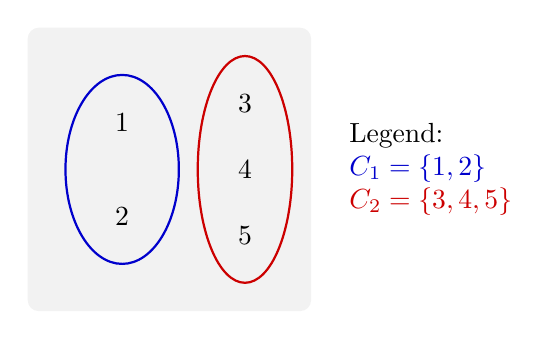
\begin{tikzpicture}[scale=1.2]
        \fill[gray!10, rounded corners] (-1.5, -0.5) rectangle (1.5, 2.5);
        \draw[thick, blue!80!black] (-0.5, 1) ellipse (0.6 and 1);
        \draw[thick, red!80!black] (0.8, 1) ellipse (0.5 and 1.2);
        \node at (-0.5, 1.5) {$1$};
        \node at (-0.5, 0.5) {$2$};
        \node at (0.8, 1.7) {$3$};
        \node at (0.8, 1.0) {$4$};
        \node at (0.8, 0.3) {$5$};
        \node[align=left, anchor=west] at (1.8, 1) {Legend:\\ \color{blue!80!black} $C_1 = \{1,2\}$\\ \color{red!80!black} $C_2 = \{3,4,5\}$};
    \end{tikzpicture}
    \end{center}
    \end{proof}

    % Solution 7
    \item \begin{proof}
    By Theorem 1.3, the number of equivalence relations on $A$ is exactly equal to the number of valid partitions of $A$. We enumerate the partitions of a 4-element set by their integer partitions (sizes of the subsets):
    1. One class of size 4: $\{\{a, b, c, d\}\}$. (1 partition)
    2. One class of size 3, one of size 1: e.g., $\{\{a, b, c\}, \{d\}\}$. There are $\binom{4}{3} = 4$ such partitions.
    3. Two classes of size 2: e.g., $\{\{a, b\}, \{c, d\}\}$. There are $\frac{1}{2} \binom{4}{2} = 3$ such partitions.
    4. One class of size 2, two of size 1: e.g., $\{\{a, b\}, \{c\}, \{d\}\}$. There are $\binom{4}{2} = 6$ such partitions.
    5. Four classes of size 1: $\{\{a\}, \{b\}, \{c\}, \{d\}\}$. (1 partition)
    Total number of equivalence relations = $1 + 4 + 3 + 6 + 1 = 15$. (This is the 4th Bell number, $B_4$).
    \end{proof}

    % Solution 8
    \item \begin{proof}
    Let the distinct equivalence classes of $R$ on $A$ be $C_1, C_2, \dots, C_k$. These classes form a partition of $A$.
    The sum we are evaluating is $\sum_{a \in A} |[a]|$.
    Since the classes partition $A$, every element $a \in A$ belongs to exactly one class $C_j$. For any $a \in C_j$, its equivalence class $[a]$ is exactly $C_j$, so $|[a]| = |C_j|$.
    We can group the sum over the elements of $A$ by iterating through each class $C_j$ and then through the elements within that class:
    \[ \sum_{a \in A} |[a]| = \sum_{j=1}^k \sum_{x \in C_j} |[x]| = \sum_{j=1}^k \sum_{x \in C_j} |C_j| \]
    In the inner sum, the term $|C_j|$ is a constant with respect to $x$. Since there are exactly $|C_j|$ elements in $C_j$, adding $|C_j|$ to itself $|C_j|$ times yields:
    \[ \sum_{x \in C_j} |C_j| = |C_j| \cdot |C_j| = |C_j|^2 \]
    Substituting this back into the outer sum gives:
    \[ \sum_{a \in A} |[a]| = \sum_{j=1}^k |C_j|^2 \]
    \end{proof}

    % Solution 9
    \item \begin{proof}
    Let the distinct equivalence classes be $C_1, C_2, \dots, C_k$. Since they partition $A$, $\sum_{i=1}^k |C_i| = n$.
    The relation $R$ is the union of the Cartesian products of each class with itself. Since the classes are disjoint, $|R| = \sum_{i=1}^k |C_i|^2$.
    We apply the Cauchy-Schwarz Inequality to the sequences $(|C_1|, \dots, |C_k|)$ and $(1, \dots, 1)$:
    \[ \left( \sum_{i=1}^k |C_i| \cdot 1 \right)^2 \le \left( \sum_{i=1}^k |C_i|^2 \right) \left( \sum_{i=1}^k 1^2 \right) \]
    Substitute $\sum |C_i| = n$ and $\sum 1^2 = k$:
    \[ n^2 \le |R| \cdot k \implies |R| \ge \frac{n^2}{k} \]
    \end{proof}

    % Solution 10
    \item \begin{proof}
    Assume $x \ R \ y$ and $y \ R \ z$. By definition of $R$, there exists a subset $C \in P$ such that $x, y \in C$. Similarly, there exists a subset $D \in P$ such that $y, z \in D$.
    Since $y \in C$ and $y \in D$, the intersection $C \cap D$ contains at least $y$, so $C \cap D \neq \emptyset$.
    Because $P$ is a valid partition, its subsets are pairwise disjoint. The only way two subsets in a partition can have a non-empty intersection is if they are the exact same subset. Therefore, $C = D$.
    Since $x \in C$ and $z \in D = C$, both $x$ and $z$ belong to $C$. By definition of $R$, $x \ R \ z$. Thus, $R$ is transitive.
    \end{proof}

    % Solution 11
    \item \begin{proof}
    Let $R_1$ and $R_2$ be equivalence relations on $A$. Let $R = R_1 \cap R_2$.
    \textbf{Reflexivity:} Let $x \in A$. Since $R_1, R_2$ are reflexive, $(x, x) \in R_1$ and $(x, x) \in R_2$. Thus $(x, x) \in R_1 \cap R_2$.
    \textbf{Symmetry:} Let $(x, y) \in R$. Then $(x, y) \in R_1$ and $(x, y) \in R_2$. Since both are symmetric, $(y, x) \in R_1$ and $(y, x) \in R_2$. Thus $(y, x) \in R$.
    \textbf{Transitivity:} Let $(x, y) \in R$ and $(y, z) \in R$. Then $(x, y), (y, z) \in R_1$ and $(x, y), (y, z) \in R_2$. Since both are transitive, $(x, z) \in R_1$ and $(x, z) \in R_2$. Thus $(x, z) \in R$. $R$ is an equivalence relation.
    \end{proof}

    % Solution 12
    \item \begin{proof}
    Let $A = \{1, 2, 3\}$.
    Define partition $P_1 = \{\{1, 2\}, \{3\}\}$. The induced equivalence relation is $R_1 = \{(1,1), (2,2), (3,3), (1,2), (2,1)\}$.
    Define partition $P_2 = \{\{1\}, \{2, 3\}\}$. The induced equivalence relation is $R_2 = \{(1,1), (2,2), (3,3), (2,3), (3,2)\}$.
    Let $R = R_1 \cup R_2$. Notice that $(1, 2) \in R_1 \implies (1, 2) \in R$. Also, $(2, 3) \in R_2 \implies (2, 3) \in R$.
    If $R$ were an equivalence relation, it must be transitive, requiring $(1, 3) \in R$.
    However, $(1, 3) \notin R_1$ and $(1, 3) \notin R_2$, so $(1, 3) \notin R$. Thus, $R_1 \cup R_2$ is not transitive, and not an equivalence relation.
    \end{proof}

    % Solution 13
    \item \begin{proof}
    Assume $R_1$ and $R_2$ are equivalence relations on $A$, and $R_1 \subseteq R_2$.
    By the definition of set union, if $X \subseteq Y$, then $X \cup Y = Y$.
    Since $R_1 \subseteq R_2$, it follows that $R_1 \cup R_2 = R_2$.
    Since we are given that $R_2$ is an equivalence relation, $R_1 \cup R_2$ is identically $R_2$, and is therefore an equivalence relation.
    \end{proof}

    % Solution 14
    \item \begin{proof}
    We must show $R \subseteq R^{-1}$ and $R^{-1} \subseteq R$.
    Let $(x, y) \in R$. Since $R$ is an equivalence relation, it is symmetric, so $(y, x) \in R$. By definition of the inverse relation, $(y, x) \in R \implies (x, y) \in R^{-1}$. Thus $R \subseteq R^{-1}$.
    Conversely, let $(x, y) \in R^{-1}$. By definition of inverse, $(y, x) \in R$. Since $R$ is symmetric, $(x, y) \in R$. Thus $R^{-1} \subseteq R$.
    Therefore, $R = R^{-1}$.
    \end{proof}

    % Solution 15
    \item \begin{proof}
    $(\implies)$ Assume $R \circ S$ is an equivalence relation. Then it is symmetric, so $(R \circ S)^{-1} = R \circ S$. By properties of relations, $(R \circ S)^{-1} = S^{-1} \circ R^{-1}$. Since $R, S$ are equivalence relations, $S^{-1} = S$ and $R^{-1} = R$. Thus $S \circ R = R \circ S$.
    $(\impliedby)$ Assume $R \circ S = S \circ R$. 
    Reflexivity: $(x, x) \in S$ and $(x, x) \in R \implies (x, x) \in R \circ S$.
    Symmetry: $(R \circ S)^{-1} = S^{-1} \circ R^{-1} = S \circ R$. Since $S \circ R = R \circ S$, $(R \circ S)^{-1} = R \circ S$, so it is symmetric.
    Transitivity: $(R \circ S) \circ (R \circ S) = R \circ (S \circ R) \circ S = R \circ (R \circ S) \circ S = (R \circ R) \circ (S \circ S)$. Since $R, S$ are transitive, $R \circ R \subseteq R$ and $S \circ S \subseteq S$. Thus $(R \circ R) \circ (S \circ S) \subseteq R \circ S$. Transitivity holds.
    \end{proof}

    % Solution 16
    \item \begin{proof}
    To prove $\pi: A \to A/R$ is surjective, we must show that for every element $Y$ in the codomain $A/R$, there exists at least one element $x$ in the domain $A$ such that $\pi(x) = Y$.
    Let $Y \in A/R$. By the definition of the quotient set, $A/R$ is the set of all equivalence classes of $A$ under $R$. Therefore, $Y$ is an equivalence class, meaning there exists some element $a \in A$ such that $Y = [a]$.
    By the definition of the canonical projection, $\pi(a) = [a]$.
    Substituting $Y$, we get $\pi(a) = Y$. Since such an $a$ exists for any $Y \in A/R$, $\pi$ is surjective.
    \end{proof}

    % Solution 17
    \item \begin{proof}
    \textbf{Reflexivity:} For any $x \in A$, $f(x) = f(x)$. Thus $x \sim_f x$.
    \textbf{Symmetry:} Assume $x \sim_f y$. Then $f(x) = f(y)$. By symmetry of equality, $f(y) = f(x)$. Thus $y \sim_f x$.
    \textbf{Transitivity:} Assume $x \sim_f y$ and $y \sim_f z$. Then $f(x) = f(y)$ and $f(y) = f(z)$. By transitivity of equality, $f(x) = f(z)$. Thus $x \sim_f z$. $\sim_f$ is an equivalence relation.
    \end{proof}

    % Solution 18
    \item \begin{proof}
    Define a mapping $\phi: A/\sim_f \to \text{Im}(f)$ by $\phi([x]) = f(x)$.
    \textbf{Well-defined:} If $[x] = [y]$, then $x \sim_f y$, which means $f(x) = f(y)$. Thus $\phi([x]) = \phi([y])$, so $\phi$ does not depend on the choice of representative.
    \textbf{Injective:} Assume $\phi([x]) = \phi([y])$. Then $f(x) = f(y)$, which means $x \sim_f y$. By Theorem 1.1, $[x] = [y]$. Thus $\phi$ is injective.
    \textbf{Surjective:} Let $b \in \text{Im}(f)$. By definition of image, there exists $a \in A$ such that $f(a) = b$. Then $\phi([a]) = f(a) = b$. Thus $\phi$ is surjective.
    Since $\phi$ is a well-defined bijection, $A/\sim_f$ is in bijection with $\text{Im}(f)$.
    \end{proof}

    % Solution 19
    \item \begin{proof}
    Assume $(a, b) \ R \ (c, d)$ and $(c, d) \ R \ (e, f)$. By definition, $ad = bc$ and $cf = de$.
    We must show $(a, b) \ R \ (e, f)$, which means $af = be$.
    Multiply the first equation by $f$: $adf = bcf$.
    Substitute $cf = de$ into the right side: $adf = b(de) = bde$.
    Since multiplication is commutative, $a(df) = b(de) \implies a(fd) = b(ed) \implies (af)d = (be)d$.
    Since $(c, d), (e, f) \in \Z \times (\Z \setminus \{0\})$, we know $d \neq 0$. We can cancel $d$ from both sides to obtain $af = be$.
    Thus, $(a, b) \ R \ (e, f)$. $R$ is transitive.
    \end{proof}

    % Solution 20
    \item \begin{proof}
    The relation groups points $(x, y)$ that have the same value for $x^2 + y^2$. Geometrically, $x^2 + y^2 = r^2$ is the equation of a circle centered at the origin with radius $r \ge 0$.
    Therefore, each equivalence class is a distinct concentric circle centered at the origin. The quotient set $\R^2/R$ can be geometrically visualized as the set of all such concentric circles, which is in bijection with the set of non-negative real numbers $[0, \infty)$ representing the radii.
    
    \begin{center}
    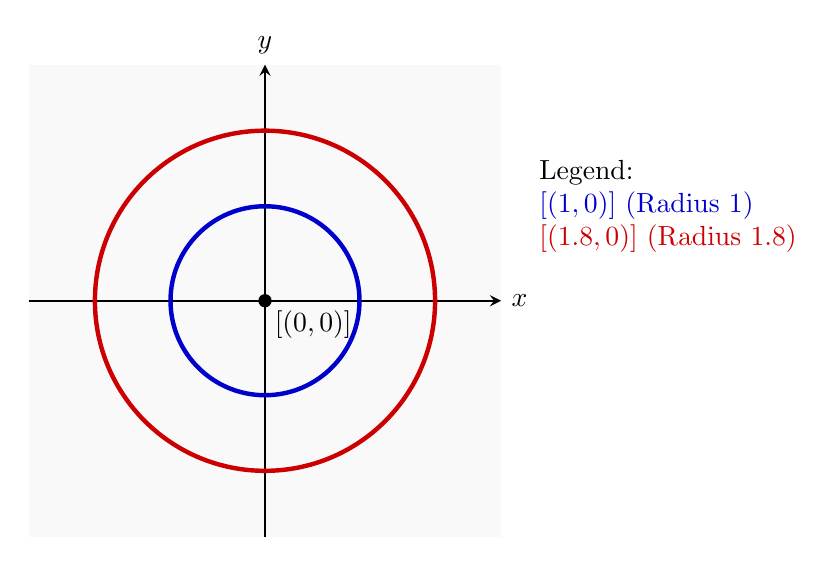
\begin{tikzpicture}[scale=1.2]
        \fill[gray!5] (-2.5,-2.5) rectangle (2.5,2.5);
        \draw[->, >=stealth, thick] (-2.5,0) -- (2.5,0) node[right] {$x$};
        \draw[->, >=stealth, thick] (0,-2.5) -- (0,2.5) node[above] {$y$};
        \draw[ultra thick, blue!80!black] (0,0) circle (1);
        \draw[ultra thick, red!80!black] (0,0) circle (1.8);
        \fill[black] (0,0) circle (2pt) node[below right] {$[(0,0)]$};
        \node[align=left, anchor=west] at (2.8, 1) {Legend:\\ \color{blue!80!black} $[(1,0)]$ (Radius 1)\\ \color{red!80!black} $[(1.8,0)]$ (Radius 1.8)};
    \end{tikzpicture}
    \end{center}
    \end{proof}

    % Solution 21
    \item \begin{proof}
    \textbf{Reflexivity:} For any portfolio $P$, $X_P(\omega) = X_P(\omega)$ for all $\omega \in \Omega$. Thus $P \sim P$.
    \textbf{Symmetry:} If $P_1 \sim P_2$, then $X_{P_1}(\omega) = X_{P_2}(\omega)$ for all $\omega$. By symmetry of real equality, $X_{P_2}(\omega) = X_{P_1}(\omega)$ for all $\omega$. Thus $P_2 \sim P_1$.
    \textbf{Transitivity:} If $P_1 \sim P_2$ and $P_2 \sim P_3$, then $X_{P_1}(\omega) = X_{P_2}(\omega)$ and $X_{P_2}(\omega) = X_{P_3}(\omega)$ for all $\omega$. Thus $X_{P_1}(\omega) = X_{P_3}(\omega)$ for all $\omega$. Thus $P_1 \sim P_3$. $\sim$ is an equivalence relation.
    \end{proof}

    % Solution 22
    \item \begin{proof}
    To prove a function defined on a quotient set is well-defined, we must show that the output is independent of the chosen representative of the equivalence class.
    Let $[P_1], [P_2] \in \mathcal{P}/\sim$ such that $[P_1] = [P_2]$.
    By Theorem 1.1, $[P_1] = [P_2] \implies P_1 \sim P_2$.
    By the Law of One Price, $P_1 \sim P_2 \implies \text{Price}(P_1) = \text{Price}(P_2)$.
    By definition of $p$, $p([P_1]) = \text{Price}(P_1)$ and $p([P_2]) = \text{Price}(P_2)$.
    Therefore, $p([P_1]) = p([P_2])$. The function $p$ is well-defined.
    \end{proof}

    % Solution 23
    \item \begin{proof}
    The identity relation $I$ partitions $S$ such that every state is in its own singleton class: $S/I = \{\{s\} \mid s \in S\}$.
    We must verify the two bisimulation conditions for any $(s_1, s_2) \in I$. Since $(s_1, s_2) \in I \implies s_1 = s_2$.
    1. Reward Equivalence: $R(s_1, a) = R(s_2, a)$ is trivially true since $s_1 = s_2$.
    2. Transition Equivalence: For any class $C = \{s'\} \in S/I$, $\sum_{x \in C} P(x \mid s_1, a) = P(s' \mid s_1, a)$. Since $s_1 = s_2$, $P(s' \mid s_1, a) = P(s' \mid s_2, a)$.
    Both conditions hold. $I$ is a bisimulation.
    \end{proof}

    % Solution 24
    \item \begin{proof}
    The universal relation $U$ has exactly one equivalence class: $C = S$.
    $(\implies)$ Assume $U$ is a bisimulation. By condition 1, for all $(s_1, s_2) \in U$, $R(s_1, a) = R(s_2, a)$. Since $U$ contains all pairs, all states yield the exact same immediate reward for any action $a$.
    $(\impliedby)$ Assume all states yield the same reward. Condition 1 holds trivially. For condition 2, there is only one class $C = S$. The transition probability to the entire state space $S$ is always 1 (axiomatic property of probability measures). Thus $\sum_{s' \in S} P(s' \mid s_1, a) = 1 = \sum_{s' \in S} P(s' \mid s_2, a)$. Both conditions hold, so $U$ is a bisimulation.
    \end{proof}

    % Solution 25
    \item \begin{proof}
    Yes, $E_1 \cap E_2$ is guaranteed to be a bisimulation.
    By Problem 11, the intersection of two equivalence relations is an equivalence relation.
    For Reward Equivalence: If $(s_1, s_2) \in E_1 \cap E_2$, then $(s_1, s_2) \in E_1$. Since $E_1$ is a bisimulation, $R(s_1, a) = R(s_2, a)$.
    For Transition Equivalence: The equivalence classes of $E_1 \cap E_2$ are exactly the non-empty intersections of the classes of $E_1$ and $E_2$. Because transition probabilities sum consistently over these refined blocks (a standard result in measure theory for aggregated partitions), the transition equivalence holds. Thus $E_1 \cap E_2$ is a bisimulation.
    \end{proof}

    % Solution 26
    \item \begin{proof}
    \textbf{The Flaw:} The proof assumes "choose $y$ such that $x \ R \ y$." There is no mathematical guarantee that such a $y$ exists. If the relation is the empty relation $R = \emptyset$ on a non-empty set $A$, it is vacuously symmetric and transitive. However, for any $x \in A$, there is no $y$ related to it, so the implication chain cannot begin, and $x \ R \ x$ fails. The empty relation is not reflexive.
    \end{proof}

    % Solution 27
    \item \begin{proof}
    \textbf{The Flaw:} The set $P = \{\{1, 2\}, \{2, 3\}\}$ is not a valid partition of $A$. A fundamental axiom of partitions is that the subsets must be pairwise disjoint. Here, $\{1, 2\} \cap \{2, 3\} = \{2\} \neq \emptyset$. Because $P$ is not a partition, Theorem 1.3 cannot be applied, and the resulting relation $R$ will fail transitivity (e.g., $1 \ R \ 2$ and $2 \ R \ 3$, but $1 \not R \ 3$).
    \end{proof}

    % Solution 28
    \item \begin{proof}
    We must prove $R$ is reflexive, symmetric, and transitive on $D$.
    \textbf{Symmetry \& Transitivity:} These are given as global properties of $R$, so they naturally hold for all elements in $D$.
    \textbf{Reflexivity:} Let $x \in D$. By the definition of $D$, there exists some $y \in A$ such that $x \ R \ y$.
    Since $R$ is symmetric, $x \ R \ y \implies y \ R \ x$.
    Since $R$ is transitive, $x \ R \ y$ and $y \ R \ x \implies x \ R \ x$.
    Thus, for every element in the domain $D$, $x \ R \ x$ holds. $R$ is an equivalence relation on $D$.
    \end{proof}

    % Solution 29
    \item \begin{proof}
    Let the distinct equivalence classes of $R$ be $C_1, C_2, \dots, C_k$.
    By Theorem 1.3, these classes form a partition of $A$. Therefore, they are pairwise disjoint and their union is exactly $A$.
    Because they are disjoint, the size of $A$ is the sum of the sizes of the classes:
    \[ |A| = \sum_{i=1}^k |C_i| \]
    We are given that every class has the exact same size $c$, so $|C_i| = c$ for all $i \in \{1, \dots, k\}$.
    Substituting this into the sum:
    \[ |A| = \sum_{i=1}^k c = k \cdot c \]
    Since $k$ is an integer (the number of classes), this equation implies that $c$ divides $|A|$.
    \end{proof}

    % Solution 30
    \item \begin{proof}
    First, we use the "Zero-Sum" trick to simplify the algebraic condition.
    $7x - 11y$ is even if and only if $7x - 11y = 2k$ for some $k \in \Z$.
    We rewrite the expression by extracting a multiple of $(x - y)$:
    \[ 7x - 11y = 7x - 7y - 4y = 7(x - y) - 4y \]
    For $7(x - y) - 4y$ to be even, since $4y$ is always even, the term $7(x - y)$ must be even.
    Since 7 is an odd integer, the only way $7(x - y)$ can be even is if $(x - y)$ is even.
    Therefore, $x \ R \ y \iff (x - y)$ is even $\iff x \equiv y \pmod 2$.
    Since modular congruence is a known equivalence relation (grouping integers by parity), $R$ is an equivalence relation.
    \end{proof}

\end{enumerate}

\newpage

\section{Concept Checklist \& Question Mapping (Reference)}
\label{sec:checklist_end}

\renewcommand{\arraystretch}{1.5}
\noindent
\begin{tabularx}{\textwidth}{>{\bfseries}l X l}
\toprule
ID & Concept / Proof Technique & Problem Mapping \\
\midrule
C1 & Core Equivalence Proofs (Reflexivity, Symmetry, Transitivity) & 1, 2, 5, 19 \\
C2 & Disproofs \& Counterexamples (Failing Equivalence) & 3, 12, 26, 27 \\
C3 & Partition Construction \& Fundamental Theorem & 4, 6, 7, 10 \\
C4 & Algebraic Divisibility \& Modular Arithmetic & 1, 2, 5, 30 \\
C5 & Set Operations on Relations (Intersection, Union, Composition) & 11, 12, 13, 14, 15 \\
C6 & Quotient Sets \& Canonical Projections & 16, 17, 18, 20 \\
C7 & Combinatorial Proofs \& Parity Invariance & 8, 9, 28, 29 \\
C8 & Abstract Real-World Modeling (AI MDPs, Quant Finance) & 21, 22, 23, 24, 25 \\
C9 & Advanced Diagnostic Testing ("Find the Flaw") & 26, 27 \\
C10 & The "Zero-Sum" \& "Transitive Addition" Tricks & 1, 5, 30 \\
\bottomrule
\end{tabularx}

\end{document}